

\section{Making Simple Queries}
\subsection{Matching RDF Literals}
\label{fig:rdf literal example} shows an example of the data graph 
\begin{figure}[htp]\centering
\caption{matching RDF literal example}
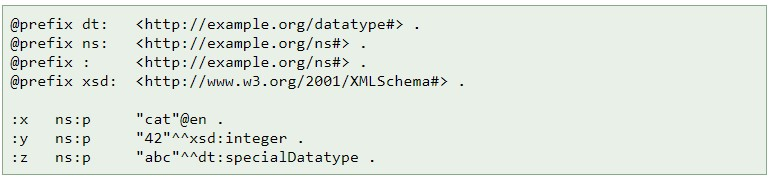
\includegraphics[scale=0.8]{langsci/img/rdfLiteralExample.jpg}
\label{fig:rdf literal example}
\end{figure} 
\subsubsection{Matching Literals with Language Tags}
Language tags in SPARQL are expressed using @ and the language tag.
This following query has no solution because "cat" is not the same RDF literal as "cat"@en:
\begin{verbatim}
SELECT ?x WHERE {?v ?p "cat"}
\end{verbatim}
but the query below will find a solution where variable is bound to :x because the language tag is specified and matches the givend data:
\begin{verbatim}
SELECT ?v WHERE {?v ?p "cat"@en}
\end{verbatim}
the result is:
\begin{verbatim}
 v
 <http://example.org/ns#x>
\end{verbatim}

\subsubsection{Matching Literals with Numeric Types}
Integers in a SPARQL query indicate an RDF typed literal with the datatype xsd:integer. For exmple: 42 is a shorteded form of 
\begin{verbatim}
"42"^^<http://www.w3.org/2001/XMLSchema#integer>
\end{verbatim}
\subsection{Creating Values With Expessions}
SparQL 1.1 allows to create values from complex expressions. The queries below show how to the \textcolor{blue}{CONCAT} function can be used to concatenate first names and last names from foaf data, then assign the value usig an \textcolor{blue}{expression in the SELECT clause} and also assign the value by using the \textcolor{blue}{BIND} form.
Data:
\begin{fullgreenverb}
@prefix foaf:  <http://xmlns.com/foaf/0.1/> .
      
_:a  foaf:givenName   "John" .
_:a  foaf:surname  "Doe" .
\end{fullgreenverb}

Query:
\begin{fullblueverb}
PREFIX foaf:   <http://xmlns.com/foaf/0.1/>
SELECT ( CONCAT(?G, " ", ?S) AS ?name )
WHERE  { ?P foaf:givenName ?G ; foaf:surname ?S }
\end{fullblueverb}

Query:
\begin{fullblueverb}
PREFIX foaf:   <http://xmlns.com/foaf/0.1/>
SELECT ?name
WHERE  { 
  ?P foaf:givenName ?G ; 
     foaf:surname ?S 
BIND(CONCAT(?G, " ", ?S) AS ?name)
}
\end{fullblueverb}
And then the result for those two queries are the same:
\begin{fullgrayverb}
name
"John Doe"
\end{fullgrayverb}

